\section{Index metrics}

\subsection{Theoretical framework}
 
Each individual indicator (or sub-indicator) addresses a different aspect of the state of an
ecosystem.  Hence, even a modest number of (sub)indicators will yield multiple perspectives on
ecosystem health.  Capturing the essence of the ecosystem health or an indicator thereof,
necessitates integrating (aggregating) each of these perspectives together into a single
\textit{index}.  There are numerous methods that have been applied to index aggregation, the most
popular of which are itemized by \citet{Fox-2013-2013} and described and evaluated in the context of
water quality indices by either \citet{Walsh-2012} (from the perspective of cost benefit analyses)
or \citet{Whittaker-2012}.

\subsubsection{Multivariate health indicators}

Motivated by the need to integrate multiple disparately scaled ecological variables together in the
absence of any normalizing information (such as benchmarks, guidelines or thresholds, see Section
\ref{sec:benchmarks}), a variety of predominantly multivariate analyses have been used in the
generation of ecosystem health indices.  However, \citet{Whittaker-2012} cautioned that since the
incorporated weights are all exclusively informed by the statistical properties of the constituent
indicator data, if these statistical properties did not coincide with expert knowledge of the
relative importance of the indicators, then the resulting indices are likely to be poor.

As an alternative, \citet{Whittaker-2012} suggest the Malmquist index.  The computational details of
the Marlmquist index are rather complex and since this method does not appear to have been adopted
by any report cards, we will restrict our description to just a brief overview.
\citet{Whittaker-2012}'s proposed version of the Malmquist index calculates pairwise ratios of
indicator distances from a multivariate benchmark curve.  The benchmark curve (a form of
indifference curve), is a multivariate curve defined by the lower boundary of a convex hull of all
indicator values and is thus derived entirely from the observed data.  Using simulated data with
manufactured statistical complications (heterogeneity and temporal autocorrelation),
\citet{Whittaker-2012} demonstrated that the Malmquist index out performs indices based on principal
components analysis and suggested other statistical methods would have similar shortcomings.

\subsubsection{Thresholds}\label{sec:benchmarks}

The absolute value of an indicator is rarely a meaningful assessment of ecosystem health
assessments.  Nor are the statistical properties of a time series necessarily a good basis for
normalizing indicators or representing the objectives.  What constitutes a 'good' or 'poor' level is
likely to vary according to indicator, the ecosystem (e.g. freshwater, estuarine or marine) as well
as the geographical and temporal (e.g. pre-industrial or current, seasonal) context.  Another way to
normalize the location (center) of indicators (if not the scale as well) that incorporates both
knowledge about the ecological basis of the indicator and the objectives that they address is to
express the indicators relative to \textit{benchmarks}.

Benchmarks are typically either reference or baseline conditions (sites or historic data
representing relatively low disturbance 'healthy' conditions), threshold values (ecotoxicology
tolerances representing the cusp of 'unhealthy conditions) or guideline values (derived from either
historical quantiles or ecotoxicology).  Thresholds and guideline values are typically peer reviewed
and ecologically meaningful, yet their specificity varies from local to regional, national or
international standards.
 
Whilst a `distance to benchmark' approach does provides some level of standardization
\citep{Connolly-2013}, to be useful, not only should there be some form of homogenization in what
the benchmark condition represents, the polarity of the distance should be well understood
\citep{Hijuelos-2013} and the magnitude of the distance should be commensurate with position along a
disturbance gradient.  That is, there should be some consistency in what it means to be above or
below a benchmark, and indeed what it means to be a certain distance from a benchmark.  Ideally,
benchmarks should also be locally relevant \citep{Connolly-2013} and consider seasonal variability
\citep{Coates-2007, Hallett-2012}.  Indeed, in a review of the methodologies used to set benchmarks,
\citep{Borja-2012} demonstrated the importance of setting appropriate benchmarks from which to
assess ecosystem quality by directly linking the inability of indices to detect impacts in
ecosystems to inappropriate reference conditions.

It is also important that benchmarks align with objectives in order to ensure indicators are
appropriate.  For example, if an objective is to maintain sustainable stocks of a particular species
of fish, a benchmarks that reflect either historical numbers or the numbers present at low pressure
sites do not necessarily represent the level of sustainability.

Ecological monitors have long recognized the need to express ecosystem ratings as standardized
scores and in terms that are more accessible to policy makers and the general public.  Whilst
initial applications focused on normalizing observed measures against subjective rating curves to
yield dimensionless index values on the scale of [0,1] that could be readiby combined into a single
understandable score or rating \citep[e.g.][]{Miller-1986}, more recent studies have explored
formulations that compare observed measures to baseline, reference, objectives or guideline values
(collectively, benchmarks) values \citep[e.g.][]{CCME-2001, Hurley-2012-3544, Jones-2013}.

\citet{Connolly-2013} reviewed the use of report cards for monitoring ecosystem health and tabulated
the general properties of a range of methods employed across a many different monitoring programs.
Rather than duplicate that information here, the current intention is to provide more specific
details about the algorithms used across those programs.

\subsubsection{Unifying indices}\label{sec:unifyingIndices}

The Canadian Council of Ministers of the Environment Water Quality Index \citep[CCME
WQI;][]{CCME-2001} incorporates comparisons to baseline based on \textit{scope} (proportion of
indicators that have one or more failures to meet objectives), \textit{frequency} (proportion of all
comparisons failing to meet objectives) and \textit{amplitude} (the normalized degree to which
failed comparisons exceed objectives).

$$
\begin{flalign*} F_1 &=
100.\bigg(\frac{Number~of~failed~indicators}{Total~number~of~indicators}\bigg)\\ F_2 &=
100.\bigg(\frac{Number~of~failed~comparisons}{Total~number~of~comparisons}\bigg)\\ F_3 &=
\frac{100.E}{1+E};\hspace{1cm} E=\frac{\sum^n_{i=1} e_i}{n};\hspace{1cm} e_i
=z_i.\left[\bigg(\frac{x_i}{benchmark_i}\bigg)^{\lambda_i} - 1\right]\\ z_i &= \begin{cases} 1 &
\text{if ith comparison fails}\\ 0 & \text{otherwise}
\end{cases}; \hspace{1cm} \lambda_1 = \begin{cases} 1 & \text{If} < benchmark_i = \text{fail}\\ -1 &
\text{If} > benchmark_i = \text{fail}\\
\end{cases}\\ CCME WQI &=100-\Bigg(\frac{\sqrt{F_1^2 + F_2^2 + F_3^2}}{1.732}\Bigg)
\end{flalign*}
$$

where $n$ is the number of comparisons.


Whilst the CCME WQI might serve its purpose in the context to which it is applied, it is unlikely to
be a useful metric for any indices involving remote sensing data or indeed any situation with a
reasonable large amount of data or indicators. One-third of the weighting of the metric is
calculated on the proportion of indicators that failed.  The more observations are collected, the
more likely at least one of them will exceed the benchmark.  Hence, this one-third will quickly
approach a constant of 1 thereby reducing overall sensitivity.  In addition, the one-third of the
method that weighting on amplitude only does so with respect to failure - there is no degree of how
well the data recedes the benchmark.
Finally, unifying indices have very limited scope for
propagating any uncertainty.  Consequently, this metric of index computation will not be explored in
this project.

Rather than calculate the proportion of all comparisons failing to meet objectives across all indicators
(as in the \textit{frequency} component of the CCME WQI), we could perform the calculation separately
for each variable (measure).  Whilst this formulation (\textbf{Exceedence}), is characterised by the same limitations
as the above \textit{frequency} component, since it is calculated separately for each variable, when aggregated
together to form an overall indicator, there is greater potential for improved resolution and granularity.


\subsubsection{Hierarchical indices}\label{sec:hierarchicalIndices}

The CCME WQI unifies all indicators into a single index as part of the calculations.  However, most
other indices involve aggregating across a sets of individual indicator scores.  There are numerous
ways to formulate indicator scores based on deviations from a benchmark (see Table
\ref{tab:indexMethods}).

Importantly, these scores are typically calculated at the level of the observations.  Most of the
index formulations are relatively robust to outliers (since the scores are either on a scale that
reduces the magnitude of outliers or are capped to a range) and thus aggregating together indicies
is likely to be more robust than calculating indices from aggregated raw data.  An exception to this
might be in situations where benchmarks are defined in the context of a specific spatial or temporal
aggregation (such as annual mean or median value).

The Binary method expresses a comparison to benchmark values on a binary compliance scale (1:
complies with benchmark, 0: fails to comply) and whilst simple to perform and understand, this
method results in indices that have the potential to be either under or overly sensitive (depending
on how far observed values typically are from the benchmark).  For example, at one extreme (when
values are close to benchmark), slight changes yield dramatic fluctuations in scores.  However, when
values are substantially above or below the benchmark, even modest improvements or deterioration
will be undetected.  This rapid 'switching' behaviour is depicted by the stepped response curve.

Note, when aggregated via means, the Binary method is identical to the Exceedence method, except
that uncertaintly propagation is slightly more straight forward via the Binary method.


In the State of the Great Lakes Report \citep{EPA/EC-1995}, greater granuality is achieved via a
panel of experts who classify each of six health indicators (aquatic community health, human health,
habitat, contaminants, nutrients and economy) into four categories: poor, mixed/deteriorating,
mixed/improving, good/restored.  Similar expert rating or multi-category exceedance grading systems
are employed in other report cards \citep[e.g Tamar estuary Report Card;][]{Attard-2012} and whilst
probably reasonably accurate, they are nonetheless highly dependent on the ongoing availability of a
reasonably stable panel of independent experts.

The Benchmark and Worst Case Scenario method (see Table \ref{tab:indexMethods}) employed by the
Fitzroy Basin Report Card \citep{Jones-2013} reflects the degree of failure by scaling the
difference between the observed values and benchmarks (20$_{th}$ or 80$_{th}$ percentile of long
term data for values above and below the benchmark respectively) to the Worst Case Scenario values
(10$_{th}$ or 90$_{th}$ percentiles respectively).  The associated response curve demonstrates a
linear decline in Score with increasing distance from the benchmark.

The Modified Amplitude method calculates the distance to benchmark on a logarithmic (base 2) scale.
The base 2 logarithm represents ratios on a symmetric scale such that value that are twice and half
the benchmark yield scores of the same magnitude (yet apposing signs), and has some inbuilt capacity
to accommodate skewed data.  The Modified Amplitude response curve illustrates how this method can
be simultaneously relatively insensitive to slight fluctuations around the benchmark as well as
sensitive to changes further away from the benchmark.

Contrastingly, the Logistic Amplitude method operates on a logit scale such that it is very
sensitive to slight fluctuations close to the benchmark and becomes progressively less sensitive
with increasing distance.  This method is also automatically scaled to the range [0,1].  The
steepness of the Logistic Amplitude response can also be controlled by a tuning parameter ($T$).




Water Quality indices (which are standardized measures of condition) are typically expressed
relative to a guideline, threshold (see Table \ref{tab:thresholds} on page \pageref{tab:thresholds})
or benchmark. Of the numerous calculation methods available, those that take into account the
distance from the threshold (i.e. incorporate \emph{difference-to-reference}) rather than simply an
indication of whether or not a threshold value has been exceeded are likely to retain more
information as well as being less sensitive to small changes in condition close to the threshold.

The challenging aspect of distance (or amplitude) based index methodologies is that determinination
what constitutes a large deviation from a benchmark depends on the scale of the measure.  For
example, a deviation of 10 units might be considered relatively large of turbidity (NTU) or salinity
(ppt), yet might be considered only minor for the Chlorophyll-a ($\mu g/L$). In order to combine a
range of such metrics together into a meaningful index, the individual scores must be expressed on a
common scale.  Whilst this is automatically the case for Binary compliance, it is not necessarily
the case for distance based indices.
    
Table \ref{tab:indexMethods} describes and compares the formulations and response curves of the
Binary compliance method as well as a number of amplitude (distance based) indexing methods.

The Modified Amplitude and Logistic Modified Amplitude are both based on a base 2 logarithm of the
ratio of observed values to the associated be benchmark (see Table \ref{tab:indexMethods}).  This
scale ensures that distances to the benchmark are symmetric (in that a doubling and halving equate
to the same magnitude - yet apposing sign).  Furthermore, the logarithmic transformation does
provide some inbuilt capacity to accommodate log-normality (a common property of measured values).

By altering the sign of the exponent, the Modified Amplitude methods can facilitate stressors and
responses for which a failure to comply with a benchmark would be either above or below the
benchmark (e.g. NTU vs Secchi depth).  Further modifications can be applied to accommodate measures
in which the benchmark represents the ideal and deviations either above or below represent
increasingly poorer conditions (e.g. pH and dissolved oxygen).
  
The raw Modified Amplitude scores are relatively insensitive to small fluctuations around a
benchmarks and sensitivity increases exponentially with increasing distance to the benchmark.  The
resulting scores can take any value in the real line [$-\infty, \infty$] and hence are not
bounded\footnote{Unbounded indices are difficult to aggregate, since items that have very large
magnitude scores will have more influence on the aggregation than those items with scores of smaller
magnitude.  Furthermore, unbounded scores are difficult to convert into alphanumeric Grades.
Consequently, the Scores need to be scaled before they can be converted to alphabetical grading
scale.}  There are two broad approaches to scaling (see Table \ref{tab:indexMethods}):

\begin{enumerate}
\item Capping and scaling: The $log_2$ scale can be capped to a range representing either a constant
extent of change (e.g. twice and half the benchmark - a cap factor of 2) or else use historical
quantiles (10th and 90th percentiles) to define the upper and lower bounds to which to cap the
scale.  Note historical quantiles are unavailable for the current application\footnote{The use of
  historical quantiles makes the explicit assumption that the domain of expectations (from very good
  to very poor) is encapsulated within the historical data.  For the eReefs model data, only three
  years of historical data are available.  This is unlikely to be sufficient to represent the full
  spread of what we should consider our expectations - particularly when we acknowledge that the eReefs
  model data do not extend back as far as the 2010-2011 floods during which water quality conditions
might be expected to be lower than the years to follow.}. Thereafter, either
can be scaled to the range [0,1] via a simple formula (see Table \ref{tab:indexMethods} III.Scaled).
  
\item Logistic Modified Amplitude: By expressing the scores on a logistic scale, the range of scores
can be automatically scaled to range [0,1].  Moreover, this method allows the shape of the response
curve to be customized for purpose.  For example, the relative sensitivity to changes close or far
from the benchmarks can be altered by a tuning parameter.
\end{enumerate}

Rather than aggregating across sites before calculating indices, we would suggest that indices
should be calculated at the site level.  This is particularly important when different measures are
measured at different sites.  Spatial variability can be addressed via the use of a bootstrapping
routine (see below).  We would recommend that measurements collected throughout the reporting year
be aggregated together into a single annual value.  This is primarily because most water quality
thresholds pertain specifically to annual averages rather than single time samples. Although it is
possible to incorporate uncertainty due to temporal variability, the low sparse temporal frequency
of sample collection is likely to yield uncertainty characteristics that will swamp the more
interesting spatial sources of uncertainty.

Alternatively, if we relax the application of thresholds to individual observations, annual indices
can be generated by aggregating observations level indices.  When doing so, the Binary Compliance
formulation aggregated via means will yield identical outcomes to the Exceedence formulation.

A useful metric for comparing the sensitivity of one indexing method over another is to take some
representative longitudinal data and calculate indices based on the actual data as well as data that
introduces progressively more noise.

 
\LTcapwidth=\textwidth
 
\begin{longtable}{lll} 
\caption{Formulations and example response curves for a variety of indicator scoring methods that compare
observed values ($x_i$) to associated benchmark, thresholds or references values ($B_i$ and
dashed line). The Scaled Modified Amplitude Method can be viewed as three Steps: I. Initial Score
generation, II. Score capping (two alternatives are provided) and III. Scaling to the range
[0,1]. The first of the alternative capping formulations simply caps the Scores to set values (on a
$log_2$ scale), whereas the second formulation (Quantile based, where $Q1$ and $Q2$ are quantiles) allows thresholds quantiles to be used
for capping purposes.  Dotted lines represent capping boundaries.
In the Logistic Scaled Amplitude method, $T$ is a tuning parameter that controls the logistic rate (steepness at the inflection point).
For the purpose of example, the benchmark was set to 50.}\label{tab:indexMethods}\\[-1em]
\toprule
\textbf{Method}&\textbf{Formulation}&\textbf{Response curve}\\
\midrule
\endfirsthead
\multicolumn{3}{l}{Table \ref{tab:indexMethods}: Report Card indexing methods, continued}\\[1ex]
\toprule
\textbf{Method}&\textbf{Formulation}&\textbf{Response curve}\\
\midrule
\endhead
\specialrule{1pt}{0pt}{0pt}
\endfoot
%%%%%%%%%%%%%%%%%%%%%%%%%%%%%%%%%%%%%%%%%%%%%%%%%%%%%%%%%%%%%%%%%%%%
\parbox[c][10em][t]{5em}{Binary\\compliance}&
\parbox[c][10em][t]{23em}{
\left$$
Score_i =
\left\{
\begin{array}{l l}
1 & \text{if}~x_i \le B_i\\
0 & \text{if}~x_i~\text{else}\\
\end{array}
$$
}
&
\parbox[c][10em][t]{10em}{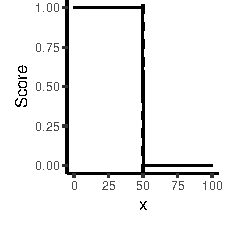
\includegraphics[]{figures/Indices/binary.pdf}}\\
\midrule
%%%%%%%%%%%%%%%%%%%%%%%%%%%%%%%%%%%%%%%%%%%%%%%%%%%%%%%%%%%%%%%%%%%%
\parbox[c][10em][t]{5em}{Benchmark and WCS}&
\parbox[c][10em][t]{23em}{
\left$$
Score_i =
\left\{
\begin{array}{l l}
100 & \text{if}~x_i \le B_i\\
0 & \text{if}~x_i \ge WCS_i\\
\left[1.0-\begin{vmatrix}\frac{x_i - B_i}{WCS_i - B_i}\end{vmatrix}\right].100 & \text{else}
\end{array}
$$
}
&
\parbox[c][10em][t]{10em}{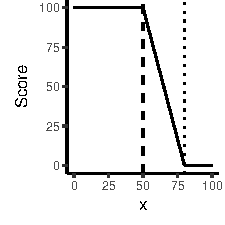
\includegraphics[]{figures/Indices/wcs.pdf}}
\\
\midrule
%%%%%%%%%%%%%%%%%%%%%%%%%%%%%%%%%%%%%%%%%%%%%%%%%%%%%%%%%%%%%%%%%%%%
\parbox[c][10em][t]{5em}{Amplitude}&
\parbox[c][10em][t]{23em}{
\left$$
Score_i = \left\{
\begin{array}{l l}
(\frac{x_i}{B_i})^{-1} & \text{if}>B_i=\text{fail}\\
(\frac{x_i}{B_i})^{1} & \text{if}<B_i=\text{fail}\\
\end{array}$\\[1em]
$Score_i = \frac{100\times Score_i}{1+Score_i}$
$$
}
&
\parbox[c][10em][t]{10em}{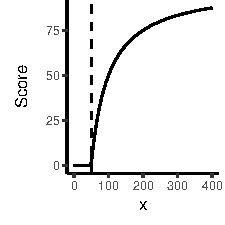
\includegraphics[]{figures/Indices/amp.pdf}}
\\
\midrule
%%%%%%%%%%%%%%%%%%%%%%%%%%%%%%%%%%%%%%%%%%%%%%%%%%%%%%%%%%%%%%%%%%%%
\parbox[c][10em][t]{5em}{Modified Amplitude}&
\parbox[c][10em][t]{23em}{
I. Raw (MAMP)\\
\left$$
Score_i = \left\{
\begin{array}{l l}
log_2(\frac{x_i}{B_i})^{-1} & \text{if}>B_i=\text{fail}\\
log_2(\frac{x_i}{B_i})^{1} & \text{if}<B_i=\text{fail}\\
\end{array}$
$$
}
&
\parbox[c][10em][t]{10em}{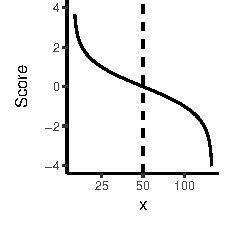
\includegraphics[]{figures/Indices/mamp.pdf}}\\
%%%%%%%%%%%%%%%%%%%%%%%%%%%%%%%%%%%%%%%%%%%%%%%%%%%%%%%%%%%%%%%%%%%%
\parbox[c][10em][t]{5em}{}&
\parbox[c][10em][t]{23em}{
II. Fixed caps (Fold=2; [0.5,2]) \textcolor{gray}{(Fold=4; [0.25,4])}\\
\left$$
Score_i = \left\{
\begin{array}{l l}
log_2(1/2) & \text{if}~Score_i < -1\\
log_2(2/1) & \text{if}~Score_i > 1\\
Score_i &otherwise\\
\end{array}$
$$
}
&
\parbox[c][10em][t]{10em}{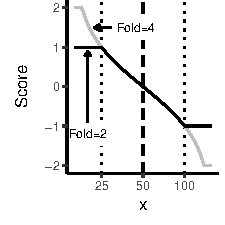
\includegraphics[]{figures/Indices/cmamp.pdf}}\\
%%%%%%%%%%%%%%%%%%%%%%%%%%%%%%%%%%%%%%%%%%%%%%%%%%%%%%%%%%%%%%%%%%%%


\parbox[c][10em][t]{5em}{}&
\parbox[c][10em][t]{23em}{
II. Quantile/extremes based caps ([15,170])\\
\left$$
Score_i = \left\{
\begin{array}{l l}
log_2(\frac{Q1}{B_i})^{-1} & \text{if}~x_i<Q1\\
log_2(\frac{Q2}{B_i})^{1} & \text{if}~x_i>Q2\\
Score_i &otherwise\\
\end{array}$
$$
}
&
\parbox[c][10em][t]{10em}{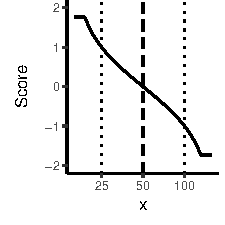
\includegraphics[]{figures/Indices/qmamp.pdf}}\\
%%%%%%%%%%%%%%%%%%%%%%%%%%%%%%%%%%%%%%%%%%%%%%%%%%%%%%%%%%%%%%%%%%%%
\parbox[c][10em][t]{5em}{}&
\parbox[c][10em][t]{23em}{
III. Scaled (Fixed: Fold=2)\\
$$
Score_i = \frac{Score_i - min(Score_i)}{max(Score_i) - min(Score_i)}
$$
}
&
\parbox[c][10em][t]{10em}{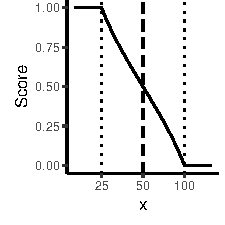
\includegraphics[]{figures/Indices/fsmamp.pdf}}\\
\midrule
%%%%%%%%%%%%%%%%%%%%%%%%%%%%%%%%%%%%%%%%%%%%%%%%%%%%%%%%%%%%%%%%%%%%
\parbox[c][10em][t]{5em}{Logistic Scaled Modified Amplitude}&
\parbox[c][10em][t]{23em}{
Raw\\
\left$$
Score_i = \left\{
\begin{array}{l l}
log_2(\frac{x_i}{B_i})^{-1} & \text{if}>B_i=\text{fail}\\
log_2(\frac{x_i}{B_i})^{1} & \text{if}<B_i=\text{fail}\\
\end{array}$\\
$Score_i = \frac{1}{1+e^{Score_i.-T}}$
$$
}
&
\parbox[c][10em][t]{10em}{\includegraphics[]{gigures/Indices/lsmamp.pdf}}\\
%%%%%%%%%%%%%%%%%%%%%%%%%%%%%%%%%%%%%%%%%%%%%%%%%%%%%%%%%%%%%%%%%%%%
\parbox[c][10em][t]{5em}{Logistic}&
\parbox[c][10em][t]{23em}{
Raw\\
\left$$
Score_i = \left\{
\begin{array}{l l}
\frac{1}{1+e^{T.(x_i/B_i)}}& \text{if}>B_i=\text{fail}\\
\frac{1}{1+e^{-T.(x_i/B_i)}}& \text{if}<B_i=\text{fail}\\
\end{array}$
$$
}
&
\parbox[c][10em][t]{10em}{\includegraphics[]{figures/Indices/lsmamp.pdf}}\\
\bottomrule
\end{longtable}



Whilst the state of the water (or other environmental condition) might be of interest in its own
right, it might also be of interest from the perspective of the ecosystem supported by the
water.  For example, turbidity might be considered to provide important insights into the
light availabity within the ecosystem.  As such, the variability in light availability (turbidity)
might be a more influential ecological driver/pressure than the exact light level within any given
time frame.  Furthermore, sustained conditions might be more influential than rapidly fluctuating
conditions.  For example, two time windows could experience the same turbidity average and variance, yet
these summaries could manifest from very different fluctuation patterns (one experiencing rapid fluctuations,
and the other experiencing sustained periods of contrasting conditions).

One index that captures the pattern of fluctuations could be based on a metric that expresses the number of
consecutive days in which a threshold has been exceeded as a proportion of number of days in the
time window (e.g. 365 days).
$$
Score_i = 1-(n_i/N_i)
$$
where $n_i$ is the maximum number of consecutive time units in which $x_i > B_i$ and $N_i$ is the number
of time units in the $i^{th}$ spatio-temporal window.

Unfortunately, such a formulation imposes some relatively difficult requirements on the data.
Firstly, the time series within each window must be complete (no gaps), otherwise it is difficult
to asses $N_i$. This requirement limits its use to only the eReefs modelled data as the Satellite
data, AIMS insitu and AIMS FLNTU data have substantial time gaps.  Secondly, as the formulation
is based on summing up exceedences, it is likely to be as susceptable to the recognised insensitivies
associated with binary compliance.  Indeed, these sensitivities may well be further amplified.
Furthermore, it is not responsive to the magnitude of exceedence.


%\subsection{Summary of adopted methodologies}

The next section will explore the performance of the following index formulations:
\begin{itemize}
  \item Binary compliance (Binary)
  \item Exceedence - proportion of observations exceeding the threshold (on large datasets, this will converge with Binaary compliance (Exceed)
  \item Maximum duration of exceedence (Max\_Duration)
  \item Modified Amplitude (MAMP)
  \item Fixed Modified Amplitude (fMAMP)
  \item Fixed Scaled (x2,1/2) Modified Amplitude (fsMAMP)
  \item Fixed Scaled (x4,1/4) Modified Amplitude (fsMAMP4)
\end{itemize}


\subsection{Index sensitivity}\label{sec:indexSensitivity}

The sensitivity of a metric can be gauged by either:
\begin{itemize}
\item Quantitative exploration of the relationships between the metric and gradients of the
underlying conditions that the metric should respond to. This approach requires very well defined
gradients as well as a clear understanding and measures of what constitutes a relationship.  By
optimizing the metric(s) to these gradients, this approach has the potential to bias outcomes
towards these gradients at the expense of generality to other gradients.
\item Have experts (or end users) qualitatively gauge the outcomes of different metrics against
expected trends and patterns.  That is, do the outcomes align with end user expectations.  Although
this approach is equally subjective and potentially biased as the quantitative exploration, it does
not necessitate formulating statistical cutoffs and associated artifacts.
\item Explore the behaviour and characteristics of the metric when calculated on data simulated to
represent a range of scenarios (altering location and spread).  Whilst this approach will not
necessarily select the 'best' metric, it does permit identification of the limitations and
assumptions associated with different metrics.
\end{itemize}

The above approaches are not mutually exclusive.  The current project will explicitly explore
sensitivity via a simulation approach, yet will also encourage feedback as to whether final outcomes
align with expectations.  It should be noted that the current project is limited in sources of data
and measured properties.  A metric is purely a re-expression of data in order to enhance or
highlight a signal.  If the underlying data do not contain the expected signal, a signal will
likewise be absent from any metrics.

To explore the performance and sensitivity of the various index computations for a range of data
scenarios, data were simulated from Gamma distributions varying in mean (relative to a threshold)
and variance and sample size.  The Gamma distribution is parameterized by two shape parameters that
can be expressed in terms of mean and variance ($Gamma(\mu^2/\sigma^2, \mu/\sigma^2)$).

For each threshold value (GL = {0.1,0.2,0.5,1,1,10,100}) and sample size (R={10,100,1000}), a set of
28 data scenarios where simulated (see Table \ref{tab:datascenarios} so as to represent a full
spectrum of possible sampling outcomes.  For each threshold/sample size and set combination, indices
were calculated and aggregated for the simulated data.  The extremes of these combinations are
presented in Figures \ref{fig:sensitivity_0.1_1000a}, \ref{fig:sensitivity_1_100a} and
\ref{fig:sensitivity_10_10a}, a more extensive set of Figures are in Appendix
\ref{app:indexSensitivity}.  For the set of simulations, the smaller the threshold, the more
variable the samples relative to the threshold.  Within each threshold, the set of 28 scenarios
thereby represent combinations of varying mean and relative variability.


\begin{table}[htbp]
\setlength{\tabcolsep}{5pt}
\caption{Index performance and sensitivity data scenarios. Data in each group are drawn from Gamma distributions whose parameterizations are based on a mean and variance.  In each case the mean is some multiple of the threshold (GL) value.
Multiples of threshold that are less than 1 result in data with greatest density below the threshold value.  Lower variances result in less varied data.}\label{tab:datascenarios}  
\scriptsize\begin{tabular}{ccc||ccc||ccc||ccc}
\toprule
Grp & Mean & SD & Grp & Mean & SD & Grp & Mean & SD & Grp & Mean & SD\\
\midrule	  
1 & $\mu = 0.2GL$ & $\sigma^2=0.1$ & 9 & $\mu = 0.75GL$ & $\sigma^2=0.1$ & 17 & $\mu = 1.5GL$ & $\sigma^2=0.1$  & 25 & $\mu = 4GL$ & $\sigma^2=0.1$\\
2 & $\mu = 0.2GL$ & $\sigma^2=0.2$ & 10& $\mu = 0.75GL$ & $\sigma^2=0.2$ & 18 & $\mu = 1.5GL$ & $\sigma^2=0.2$  & 26 & $\mu = 4GL$ & $\sigma^2=0.2$\\
3 & $\mu = 0.2GL$ & $\sigma^2=0.3$ & 11& $\mu = 0.75GL$ & $\sigma^2=0.3$ & 19 & $\mu = 1.5GL$ & $\sigma^2=0.3$  & 27 & $\mu = 4GL$ & $\sigma^2=0.3$\\
4 & $\mu = 0.2GL$ & $\sigma^2=0.5$ & 12& $\mu = 0.75GL$ & $\sigma^2=0.5$ & 20 & $\mu = 1.5GL$ & $\sigma^2=0.5$  & 28 & $\mu = 4GL$ & $\sigma^2=0.5$\\
5 & $\mu = 0.5GL$ & $\sigma^2=0.1$ & 13& $\mu = 1GL$ & $\sigma^2=0.1$ & 21 & $\mu = 2GL$ & $\sigma^2=0.1$\\
6 & $\mu = 0.5GL$ & $\sigma^2=0.2$ & 14& $\mu = 1GL$ & $\sigma^2=0.2$ & 22 & $\mu = 2GL$ & $\sigma^2=0.2$\\          
7 & $\mu = 0.5GL$ & $\sigma^2=0.3$ & 15& $\mu = 1GL$ & $\sigma^2=0.3$ & 23 & $\mu = 2GL$ & $\sigma^2=0.3$\\
8 & $\mu = 0.5GL$ & $\sigma^2=0.5$ & 16& $\mu = 1GL$ & $\sigma^2=0.5$ & 24 & $\mu = 2GL$ & $\sigma^2=0.5$\\          
\bottomrule
\end{tabular}	
\end{table}



\begin{figure}[h]
  \includegraphics[width=0.9\linewidth]{{figures/Sensitivity of indices/sensitivity.Group_1.GL_0.1.R_1000\res}.pdf}
  \caption{Simulated data and associated indices for threshold of 0.1 and very large sample sizes (R=1000).  Samples represent high variability relative to threshold.}\label{fig:sensitivity_0.1_1000a}
\end{figure}
\begin{figure}[h]
  \includegraphics[width=0.9\linewidth]{{figures/Sensitivity of indices/sensitivity.Group_1.GL_10.R_1000\res}.pdf}
  \caption{Simulated data and associated indices for threshold of 10 and very large sample sizes (R=1000).}\label{fig:sensitivity_10_1000a}
\end{figure}
\begin{figure}[h]
  \includegraphics[width=0.9\linewidth]{{figures/Sensitivity of indices/sensitivity.Group_1.GL_100.R_1000\res}.pdf}
  \caption{Simulated data and associated indices for threshold of 100 and very large sample sizes (R=1000).}\label{fig:sensitivity_100_1000a}
\end{figure}
\begin{figure}[h]
  \includegraphics[width=0.9\linewidth]{{figures/Sensitivity of indices/sensitivity.Group_1.GL_1.R_10\res}.pdf}
  \caption{Simulated data and associated indices for threshold of 1 and large sample sizes (R=100).}\label{fig:sensitivity_1_100a}
\end{figure} 
\begin{figure}[h]
  \includegraphics[width=0.9\linewidth]{{figures/Sensitivity of indices/sensitivity.Group_1.GL_10.R_10\res}.pdf}
  \caption{Simulated data and associated indices for threshold of 10 and small sample sizes (R=10).}\label{fig:sensitivity_10_10a}
\end{figure}
 

As expected, indices decline with increasing values relative to the threshold (as would be the case
for Chl-a or TSS) with a generally linear response being the attribute sought in our specific
context.  Testing the responses of indices to various combinations allowed the identification of the
most appropriate and robust index calculation method.

When the number of samples and the relative sample variability is very large
(e.g. fig.~\ref{fig:sensitivity_0.1_1000a}), with the exception of the the maximum duration of
exceedance and the uncapped and unscaled modified amplitude (MAMP) methods, the different index
calculation methods behave very similarly.  However, as the variability of the samples declines
relative to the threshold (e.g. compare figs.~\ref{fig:sensitivity_0.1_1000a},
~\ref{fig:sensitivity_10_1000a} and ~\ref{fig:sensitivity_100_1000a}), such that observations are
predominantly within twice/half the threshold value, %However, when the number of samples is small
and data is predominantly distributed between the threshold value %and twice/half this value, the
binary or frequency of exceedance methods both increasingly become simultaneously overly and under
sensitive.  The response curve of these metrics becomes less linear, whereas the linearity of the
other metrics is maintained for a greater span of observation means.  This is further exacerbated by
small sample sizes (see fig.\ref{fig:sensitivity_10_10a}).

Over all of the scenarios, the fsMAMP4 (Modified Amplitude capped at four times/quarter of threshold
values) appears to be as linear or more linear than the fsMAMP (Modified Amplitude capped at
twice/half), particularly as relative variability declines.  However, the cost of this extended
range of sensitivity, is that it is predominantly more sensitive at the extremes and less so (at
least compared to fsMAMP) towards the mid-region (corresponding to values close to the threshold).
Arguably, it is more desirable for an index to be most sensitive around the threshold (unless there
is substantial uncertainty about the threshold value) and become progressively less sensitive at
increasing distance from the threshold - the binary and exceedence metrics are the extreme cases of
this.


The fixed capped modified amplitude (fsMAMP) index was considered the 'best' compromise between
consistent sensitivity throughout the range of scenarios and the nature of data presented in
exploratory data analyses (see Section~\ref{sec:EDA}).  It should be noted that it is possible to
modify the fsMAMP index metric to facilitate caps based on historical, biological or ecological
parameters.  It is also possible to define these parameters (an upper and lower capping) at any
spatial/temporal/measure level so as to potentially build indices that are optimized for each
measure.  Such an exercise requires extensive expert knowledge to define and justify each of the
parameters and is beyond the scope of the current project.


\clearpage

\paragraph{Summary of simulation index sensitivity exploration}
\begin{itemize}
\item Indices decline with increasing values relative to the thresholds (and for a given
variability)
\item Indices increase with increasing variability (since in Gamma distributions, this results in
more values towards lower end)
\item when R is very large, the different indicators behave similarly (except Max\_Duration and
MAMP)
\item MAMP is more susceptable to outliers
\end{itemize}

\clearpage

\subsection{Index explorations}

Before data can be combined and aggregated across the various Sources (AIMS insitu, AIMS FLNTU,
Satellite, eReefs and eReefs926) and Measures (Chlorophyll, TSS, Secchi depth and NOx), it is
important that we evaluate the likely usefulness of each Source/Measure combination.  For example, a
Measure or Source that does not vary in both time and space is not considered very informative
parameter.

Although an exploration of the patterns of spatial and temporal variation of the raw data does offer
some insights into the usefulness of a parameter, it is variation in relation to expectations
(thresholds) that are likely to be of greatest utility.  For example, a parameter might vary
substantially in time and or space and yet always be well above (or below) the threshold.  In this
situation (despite the apparent variability), with respect to the expectation domain, there is very little
(if any) variability and thus the realised utility of the parameter is low (or else the threshold is
inappropriate for the particular measure to which it is being applied).

Different parameters are measured on different scales or else have different natural background
levels.  Since variability (for example variance) is dependent on scale, parameters measured in
larger units will typically exhibit more variability in absolute terms.  Hence, in order to compare
the relative utility of different parameters, it is necessary to either express variation relative
to scale (such as coefficient of variation) or standardize the parameters.  The scaled hierarchical
index formations of Section~\ref{sec:hierarchicalIndices} (such as Binary, fsMAMP, fsMAMP4 and
logistic MAMP) are all a form of standardization which yeild scores on scales that are all bound [0,1].

The following three subsections will provide information to assist in the selection of:
\begin{itemize}
\item which Index formulation to adopt
\item which Sources of data to use
\item which Measures to include
\end{itemize}

%Preliminary exploratory data analysis suggested that

\subsubsection{Indices}

Theoretical sensitivity investigation suggested that the fixed capped (half/twice threshold)
Modified Amplitude (fsMAMP) is likely to be the best compromise between under and over sensitivity
given the patterns of variance observed across and between the various Sources (AIMS insitu, AIMS
FLNTU, Satellite, eReefs and eReefs926) and Measures (Chlorophyll, TSS, Secchi depth and NOx).  The
alternate approach is to explore and compare the patterns of the various index formulations in the
context of both the raw collected data and expert expectations.  Broadly speaking, we might expect
that many water Quality parameters improve across the shelf with increasing distance from coastline.
We might also expect some latitudinal patterns in which water quality generally improves along a
south-north gradient with interruptions coinciding with outflow of major rivers.


To explore how the raw data are transformed into the various indices, it is useful to pair up
'before' and 'after' figures.  Again, for the sake of brevity, we will focus on the same data that
featured in Figure~\ref{fig:violin_chl_oc} (Chlorophyll-a from Wet Tropics, Open Coastal).
Figures~\ref{fig:idx.violin_chl_oc_niskin} -- \ref{fig:idx.violin_chl_oc_eReefs926} illustrate the
associations between the site means (subfigure a) and three of the major index candidates (b:
Binary, c: fsMAMP and d: fsMAMP4) for each of the Sources of data (AIMS insitu, AIMS FLNTU,
Satellite, eReefs and eReefs926).  In these figures, purple and blue lines represent annual means
and within year Generalized Additive Model \citep[][]{Wood-2006-2006} respectively and help
highlight inter- and intra-annual variation\footnote{GAMs not performed for AIMS insitu data due to
a lack of data over which to estimate splines}.

Inter and Intra annual variation is greatest in the Binary index method for each data
Source\footnote{this pattern also persists across all Zones (Region/Water body) and Measures -
although other Measures and Zones not provided here to reduce space.}.  Whilst this method does
illustrate sensitivity, the values of the index do not contain any context about the magnitude of
values relative to the threshold.  That is, it is not possible to distinguish situations in which
all observations are just under (or over) the threshold from when they are substantially under (or
over) the threshold. In this way, the index has the potential to be under-sensitive to magnitude,
yet very sensitive to change around the threshold.  For each of the Sources (except AIMS insitu for
which data are too sparse), the relative magnitude of fluctuations in the Binary index (subfigure b)
appears to be substantially greater than the relative magnitude of fluctuation in the observed data
(subfigure a).  These patterns of relative variability might imply that the Binary index is
over-sensitive.

By contrast, the fsMAMP4 (capped at four times and one-forth threshold, subfigures d) could be
interpreted as under-sensitive - particularly for the Satellite data (which has highly variable
observations).  The fsMAMP (twice/half threshold) appears to in between these two extremes and thus
could be considered a reasonable comprimise between over and under sensitivity.

Spatial representations for Wet Tropics Open Coastal Chlorophyll-a
(figs.~\ref{fig:eda.idx.spatial_chl_oc_s_niskin} -- \ref{fig:eda.idx.spatial_chl_oc_s_eReefs926})
and Dry Tropics Midshelf Chlorophyll-a (figs.~\ref{fig:eda.idx.spatial_chl_m_s_niskin} --
\ref{fig:eda.idx.spatial_chl_m_s_eReefs926}) offer similar assessments - that fsMAMP provides a
reasonable compromise between the potentially under and over sensitive fsMAMP4 and Binary
formulations.

Time series of annually aggregated observations and associated annually aggregated indices
(figs.~\ref{fig:All_sources_AIMS insitu.Annual_measure.chl_zone} --
\ref{fig:All_sources_eReefs926.Annual_measure.chl_zone}) provide simplified representations of the
overall spatio-temporal patterns.  As with the temporal and spatial representations, the fsMAMP
index consistently manifests between the Binary and fsMAMP4 formulations.

% Finally, longitudinal (figs.Additional representations

% The MAMP index capped at four times and one-quarter of the threshold (fsMAMP4) was the least variable

% - Binary index illustrates greatest sensitivity - however might be overly sensitive.
% - fsMAMP4 least sensitive
% - fsMAMP is in between
% - better descrimination around the threshold value
% - this also manifests in the spatial plots which illustrate a greater range of colors in the
%     fsMAMP than fsMAMP4
% - fsMAMP also corresponds closer to the patterns in the raw data.

% - when we explore the aggregated zone means, these same trends appear - the fsMAMP seems to be
% between the two others for all Measures and Sources. 

\begin{figure}[ptbh]
  a) AIMS insitu site means\\\includegraphics[align=t,width=0.95\linewidth]{{figures/Exploratory_Data_Analysis/Insitu/eda.year.chl_Wet Tropics__Open Coastal_niskin_log\res.pdf}}\\
  b) AIMS insitu site mean Binary\\\includegraphics[align=t,width=0.95\linewidth]{{figures/Exploratory_Data_Analysis/Insitu/eda.idx_Binary_year.chl_Wet Tropics__Open Coastal_niskin_natural\res.pdf}}\\
  c) AIMS insitu site mean fsMAMP\\\includegraphics[align=t,width=0.95\linewidth]{{figures/Exploratory_Data_Analysis/Insitu/eda.idx.year.chl_Wet Tropics__Open Coastal_niskin_natural\res.pdf}}\\
  d) AIMS insitu site mean fsMAMP4\\\includegraphics[align=t,width=0.95\linewidth]{{figures/Exploratory_Data_Analysis/Insitu/eda.idx_fsMAMP4_year.chl_Wet Tropics__Open Coastal_niskin_natural\res.pdf}}\\
  \caption{Temporal distribution of AIMS insitu Chlorophyll-a a) samples and associated b) Binary, c) fsMAMP and d) fsMAMP4 index formulations for the Wet Tropics Open Coastal zone. Red and Blue symbols represent samples collected in Dry and Wet seasons respectively.
    Green and red shaded banding on a) respectively represent half and twice threshold value (50\% shading) and one-forth and four times threshold value (30\% shading). Traffic-light banding on b-d) indicates
    simple 5-level color scheme.  Purple lines represent annual means.}\label{fig:idx.violin_chl_oc_niskin}
\end{figure}

\begin{figure}[ptbh]
  a) AIMS FLNTU raw site means\\\includegraphics[align=t,width=0.95\linewidth]{{figures/Exploratory_Data_Analysis/FLNTU/eda.year.chl_Wet Tropics__Open Coastal_flntu_log\res.pdf}}\\
  b) AIMS FLNTU site mean Binary\\\includegraphics[align=t,width=0.95\linewidth]{{figures/Exploratory_Data_Analysis/FLNTU/eda.idx_Binary_year.chl_Wet Tropics__Open Coastal_flntu_natural\res.pdf}}\\
  c) AIMS FLNTU site mean fsMAMP\\\includegraphics[align=t,width=0.95\linewidth]{{figures/Exploratory_Data_Analysis/FLNTU/eda.idx.year.chl_Wet Tropics__Open Coastal_flntu_natural\res.pdf}}\\
  d) AIMS FLNTU site mean fsMAMP4\\\includegraphics[align=t,width=0.95\linewidth]{{figures/Exploratory_Data_Analysis/FLNTU/eda.idx_fsMAMP4_year.chl_Wet Tropics__Open Coastal_flntu_natural\res.pdf}}\\
  \caption{Temporal distribution of AIMS FLNTU Chlorophyll-a a) samples and associated b) Binary, c) fsMAMP and d) fsMAMP4 index formulations for the Wet Tropics Open Coastal zone. Red and Blue symbols represent samples collected in Dry and Wet seasons respectively.
    Green and red shaded banding on a) respectively represent half and twice threshold value (50\% shading) and one-forth and four times threshold value (30\% shading). Traffic-light banding on b-d) indicates
    simple 5-level color scheme.  Purple lines represent annual means.}\label{fig:idx.violin_chl_oc_flntu}
\end{figure}

\begin{figure}[ptbh]
  a) Satellite raw site means\\\includegraphics[align=t,width=0.95\linewidth]{{figures/Exploratory_Data_Analysis/Satellite/eda.year.chl_Wet Tropics__Open Coastal__log\res.pdf}}\\
  b) Satellite site mean Binary\\\includegraphics[align=t,width=0.95\linewidth]{{figures/Exploratory_Data_Analysis/Satellite/eda.idx_Binary_year.chl_Wet Tropics__Open Coastal__natural\res.pdf}}\\
  c) Satellite site mean fsMAMP\\\includegraphics[align=t,width=0.95\linewidth]{{figures/Exploratory_Data_Analysis/Satellite/eda.idx.year.chl_Wet Tropics__Open Coastal__natural\res.pdf}}\\
  d) Satellite site mean fsMAMP4\\\includegraphics[align=t,width=0.95\linewidth]{{figures/Exploratory_Data_Analysis/Satellite/eda.idx_fsMAMP4_year.chl_Wet Tropics__Open Coastal__natural\res.pdf}}\\
  \caption{Temporal distribution of Satellite Chlorophyll-a a) samples and associated b) Binary, c) fsMAMP and d) fsMAMP4 index formulations for the Wet Tropics Open Coastal zone. Red and Blue symbols represent samples collected in Dry and Wet seasons respectively.
    Green and red shaded banding on a) respectively represent half and twice threshold value (50\% shading) and one-forth and four times threshold value (30\% shading). Traffic-light banding on b-d) indicates
    simple 5-level color scheme.  Purple lines represent annual means.}\label{fig:idx.violin_chl_oc_satellite}
\end{figure}

\begin{figure}[ptbh]
  a) eReefs raw site means\\\includegraphics[align=t,width=0.95\linewidth]{{figures/Exploratory_Data_Analysis/eReefs/eda.year.chl_Wet Tropics__Open Coastal_eReefs_log\res.pdf}}\\
  b) eReefs site mean Binary\\\includegraphics[align=t,width=0.95\linewidth]{{figures/Exploratory_Data_Analysis/eReefs/eda.idx_Binary_year.chl_Wet Tropics__Open Coastal_eReefs_natural\res.pdf}}\\
  c) eReefs site mean fsMAMP\\\includegraphics[align=t,width=0.95\linewidth]{{figures/Exploratory_Data_Analysis/eReefs/eda.idx.year.chl_Wet Tropics__Open Coastal_eReefs_natural\res.pdf}}\\
  d) eReefs site mean fsMAMP4\\\includegraphics[align=t,width=0.95\linewidth]{{figures/Exploratory_Data_Analysis/eReefs/eda.idx_fsMAMP4_year.chl_Wet Tropics__Open Coastal_eReefs_natural\res.pdf}}\\
  \caption{Temporal distribution of eReefs Chlorophyll-a a) samples and associated b) Binary, c) fsMAMP and d) fsMAMP4 index formulations  for the Wet Tropics Open Coastal zone. Red and Blue symbols represent samples collected in Dry and Wet seasons respectively.
    Green and red shaded banding on a) respectively represent half and twice threshold value (50\% shading) and one-forth and four times threshold value (30\% shading). Traffic-light banding on b-d) indicates
    simple 5-level color scheme.  Purple lines represent annual means.}\label{fig:idx.violin_chl_oc_eReefs}
\end{figure}
 
\begin{figure}[ptbh]
  a) eReefs926 raw site means\\\includegraphics[align=t,width=0.95\linewidth]{{figures/Exploratory_Data_Analysis/eReefs926/eda.year.chl_Wet Tropics__Open Coastal_eReefs926_log\res.pdf}}\\
  b) eReefs926 site mean Binary\\\includegraphics[align=t,width=0.95\linewidth]{{figures/Exploratory_Data_Analysis/eReefs926/eda.idx_Binary_year.chl_Wet Tropics__Open Coastal_eReefs926_natural\res.pdf}}\\
  c) eReefs926 site mean fsMAMP\\\includegraphics[align=t,width=0.95\linewidth]{{figures/Exploratory_Data_Analysis/eReefs926/eda.idx.year.chl_Wet Tropics__Open Coastal_eReefs926_natural\res.pdf}}\\
  d) eReefs926 site mean fsMAMP4\\\includegraphics[align=t,width=0.95\linewidth]{{figures/Exploratory_Data_Analysis/eReefs926/eda.idx_fsMAMP4_year.chl_Wet Tropics__Open Coastal_eReefs926_natural\res.pdf}}\\
  \caption{Temporal distribution of eReefs926 Chlorophyll-a a) samples and associated b) Binary, c) fsMAMP and d) fsMAMP4 index formulations for the Wet Tropics Open Coastal zone. Red and Blue symbols represent samples collected in Dry and Wet seasons respectively.
    Green and red shaded banding on a) respectively represent half and twice threshold value (50\% shading) and one-forth and four times threshold value (30\% shading). Traffic-light banding on b-d) indicates
    simple 5-level color scheme.  Purple lines represent annual means.}\label{fig:idx.violin_chl_oc_eReefs926}
\end{figure}
   
\begin{landscape}
  \begin{figure}[ptbh]
    \begin{minipage}{0.5\linewidth}
      a) AIMS insitu raw data\\\includegraphics[align=t,width=1\linewidth]{{figures/Exploratory_Data_Analysis/Insitu/eda.spatial.year.chl_Wet Tropics__Open Coastal_niskin_logA\res.png}}\\[1em]
      c) AIMS insitu fsMAMP\\\includegraphics[align=t,width=1\linewidth]{{figures/Exploratory_Data_Analysis/Insitu/eda.idx.spatial.year.chl_Wet Tropics__Open Coastal_niskin_naturalA\res.png}}\\[1em]
    \end{minipage}
    \begin{minipage}{0.5\linewidth}
      b) AIMS insitu Binary\\\includegraphics[align=t,width=1\linewidth]{{figures/Exploratory_Data_Analysis/Insitu/eda.idx_Binary_spatial.year.chl_Wet Tropics__Open Coastal_niskin_naturalA\res.png}}\\[1em]
      d) AIMS insitu fsMAMP4\\\includegraphics[align=t,width=1\linewidth]{{figures/Exploratory_Data_Analysis/Insitu/eda.idx_fsMAMP4_spatial.year.chl_Wet Tropics__Open Coastal_niskin_naturalA\res.png}}\\[1em]
    \end{minipage}
    \caption{Spatial distribution of AIMS in situ Chlorophyll-a a) samples and associated b) Binary, c) fsMAMP and d) fsMAMP4 index formulations for the Wet Tropics Open Coastal zone.
    Color bars scaled to half (green) and twice (red) threshold value for raw data and 1 (green) and 0 (red) for Binary, fsMAMP and fsMAMP4.}\label{fig:eda.idx.spatial_chl_oc_s_niskin}
\end{figure}
\end{landscape}

\begin{landscape}
  \begin{figure}[ptbh]
    \begin{minipage}{0.5\linewidth}
      a) Satellite raw data\\\includegraphics[align=t,width=1\linewidth]{{figures/Exploratory_Data_Analysis/Satellite/eda.spatial.year.chl_Wet Tropics__Open Coastal__logA\res.png}}\\[1em]
      c) Satellite fsMAMP\\\includegraphics[align=t,width=1\linewidth]{{figures/Exploratory_Data_Analysis/Satellite/eda.idx.spatial.year.chl_Wet Tropics__Open Coastal__naturalA\res.png}}\\[1em]
    \end{minipage}
    \begin{minipage}{0.5\linewidth}
      b) Satellite Binary\\\includegraphics[align=t,width=1\linewidth]{{figures/Exploratory_Data_Analysis/Satellite/eda.idx_Binary_spatial.year.chl_Wet Tropics__Open Coastal__naturalA\res.png}}\\[1em]
      d) Satellite fsMAMP4\\\includegraphics[align=t,width=1\linewidth]{{figures/Exploratory_Data_Analysis/Satellite/eda.idx_fsMAMP4_spatial.year.chl_Wet Tropics__Open Coastal__naturalA\res.png}}\\[1em]
    \end{minipage}
  \caption{Spatial distribution of Satellite Chlorophyll-a a) samples and associated b) Binary, c) fsMAMP and d) fsMAMP4 index formulations for the Wet Tropics Open Coastal zone.
    Color bars scaled to half (green) and twice (red) threshold value for raw data and 1 (green) and 0 (red) for Binary, fsMAMP and fsMAMP4.}\label{fig:eda.idx.spatial_chl_oc_s_satellite}
\end{figure}
\end{landscape}

\begin{landscape}
  \begin{figure}[ptbh]
    \begin{minipage}{0.5\linewidth}
      a) eReefs raw data\\\includegraphics[align=t,width=1\linewidth]{{figures/Exploratory_Data_Analysis/eReefs/eda.spatial.year.chl_Wet Tropics__Open Coastal_eReefs_logA\res.png}}\\[1em]
      c) eReefs fsMAMP\\\includegraphics[align=t,width=1\linewidth]{{figures/Exploratory_Data_Analysis/eReefs/eda.idx.spatial.year.chl_Wet Tropics__Open Coastal_eReefs_naturalA\res.png}}\\[1em]
    \end{minipage}
    \begin{minipage}{0.5\linewidth}
      b) eReefs Binary\\\includegraphics[align=t,width=1\linewidth]{{figures/Exploratory_Data_Analysis/eReefs/eda.idx_Binary_spatial.year.chl_Wet Tropics__Open Coastal_eReefs_naturalA\res.png}}\\[1em]
      d) eReefs fsMAMP4\\\includegraphics[align=t,width=1\linewidth]{{figures/Exploratory_Data_Analysis/eReefs/eda.idx_fsMAMP4_spatial.year.chl_Wet Tropics__Open Coastal_eReefs_naturalA\res.png}}\\[1em]
    \end{minipage}
  %b) AIMS FLNTU\\\includegraphics[align=t,width=0.95\linewidth]{{figures/Exploratory_Data_Analysis/FLNTU/eda.spatial.year.chl_Wet Tropics__Open Coastal_flntu_logA\res.png}}\\[1em]
  \caption{Spatial distribution of eReefs Chlorophyll-a a) samples and associated b) Binary, c) fsMAMP and d) fsMAMP4 index formulations for the Wet Tropics Open Coastal zone.
    Color bars scaled to half (green) and twice (red) threshold value for raw data and 1 (green) and 0 (red) for Binary, fsMAMP and fsMAMP4.}\label{fig:eda.idx.spatial_chl_oc_s_eReefs}
\end{figure}
\end{landscape}

\begin{landscape}
  \begin{figure}[ptbh]
    \begin{minipage}{0.5\linewidth}
      a) eReefs926 raw data\\\includegraphics[align=t,width=1\linewidth]{{figures/Exploratory_Data_Analysis/eReefs926/eda.spatial.year.chl_Wet Tropics__Open Coastal_eReefs926_logA\res.png}}\\[1em]
      c) eReefs926 fsMAMP\\\includegraphics[align=t,width=1\linewidth]{{figures/Exploratory_Data_Analysis/eReefs926/eda.idx.spatial.year.chl_Wet Tropics__Open Coastal_eReefs926_naturalA\res.png}}\\[1em]
    \end{minipage}
    \begin{minipage}{0.5\linewidth}
      b) eReefs926 Binary\\\includegraphics[align=t,width=1\linewidth]{{figures/Exploratory_Data_Analysis/eReefs926/eda.idx_Binary_spatial.year.chl_Wet Tropics__Open Coastal_eReefs926_naturalA\res.png}}\\[1em]
      d) eReefs926 fsMAMP4\\\includegraphics[align=t,width=1\linewidth]{{figures/Exploratory_Data_Analysis/eReefs926/eda.idx_fsMAMP4_spatial.year.chl_Wet Tropics__Open Coastal_eReefs926_naturalA\res.png}}\\[1em]
    \end{minipage}
  %b) AIMS FLNTU\\\includegraphics[align=t,width=0.95\linewidth]{{figures/Exploratory_Data_Analysis/FLNTU/eda.spatial.year.chl_Wet Tropics__Open Coastal_flntu_logA\res.png}}\\[1em]
  \caption{Spatial distribution of eReefs926 Chlorophyll-a a) samples and associated b) Binary, c) fsMAMP and d) fsMAMP4 index formulations for the Wet Tropics Open Coastal zone.
    Color bars scaled to half (green) and twice (red) threshold value for raw data and 1 (green) and 0 (red) for Binary, fsMAMP and fsMAMP4.}\label{fig:eda.idx.spatial_chl_oc_s_eReefs926}
\end{figure}
\end{landscape}

%% Dry Tropics Midshelf

\begin{figure}[ptbh]
  a) AIMS insitu raw data\\\includegraphics[align=t,width=1\linewidth]{{figures/Exploratory_Data_Analysis/Insitu/eda.spatial.year.chl_Dry Tropics__Midshelf_niskin_logA\res.png}}\\[1em]
  b) AIMS insitu Binary\\\includegraphics[align=t,width=1\linewidth]{{figures/Exploratory_Data_Analysis/Insitu/eda.idx_Binary_spatial.year.chl_Dry Tropics__Midshelf_niskin_naturalA\res.png}}\\[1em]
  c) AIMS insitu fsMAMP\\\includegraphics[align=t,width=1\linewidth]{{figures/Exploratory_Data_Analysis/Insitu/eda.idx.spatial.year.chl_Dry Tropics__Midshelf_niskin_naturalA\res.png}}\\[1em]
  d) AIMS insitu fsMAMP4\\\includegraphics[align=t,width=1\linewidth]{{figures/Exploratory_Data_Analysis/Insitu/eda.idx_fsMAMP4_spatial.year.chl_Dry Tropics__Midshelf_niskin_naturalA\res.png}}\\[1em]
  \caption{Spatial distribution of AIMS insitu Chlorophyll-a a) samples and associated b) Binary, c) fsMAMP and d) fsMAMP4 index formulations for the Dry Tropics Midshelf zone.
    Color bars scaled to half (green) and twice (red) threshold value for raw data and 1 (green) and 0 (red) for Binary, fsMAMP and fsMAMP4.}\label{fig:eda.idx.spatial_chl_m_s_niskin}
\end{figure}


\begin{figure}[ptbh]
  a) AIMS FLNTU raw data\\\includegraphics[align=t,width=1\linewidth]{{figures/Exploratory_Data_Analysis/FLNTU/eda.spatial.year.chl_Dry Tropics__Midshelf_flntu_logA\res.png}}\\[1em]
  b) AIMS FLNTU Binary\\\includegraphics[align=t,width=1\linewidth]{{figures/Exploratory_Data_Analysis/FLNTU/eda.idx_Binary_spatial.year.chl_Dry Tropics__Midshelf_flntu_naturalA\res.png}}\\[1em]
  c) AIMS FLNTU fsMAMP\\\includegraphics[align=t,width=1\linewidth]{{figures/Exploratory_Data_Analysis/FLNTU/eda.idx.spatial.year.chl_Dry Tropics__Midshelf_flntu_naturalA\res.png}}\\[1em]
  d) AIMS FLNTU fsMAMP4\\\includegraphics[align=t,width=1\linewidth]{{figures/Exploratory_Data_Analysis/FLNTU/eda.idx_fsMAMP4_spatial.year.chl_Dry Tropics__Midshelf_flntu_naturalA\res.png}}\\[1em]
  \caption{Spatial distribution of AIMS FLNTU Chlorophyll-a a) samples and associated b) Binary, c) fsMAMP and d) fsMAMP4 index formulations for the Dry Tropics Midshelf zone.
    Color bars scaled to half (green) and twice (red) threshold value for raw data and 1 (green) and 0 (red) for Binary, fsMAMP and fsMAMP4.}\label{fig:eda.idx.spatial_chl_m_s_flntu}
\end{figure}

\begin{figure}[ptbh]
  a) Satellite raw data\\\includegraphics[align=t,width=1\linewidth]{{figures/Exploratory_Data_Analysis/Satellite/eda.spatial.year.chl_Dry Tropics__Midshelf__logA\res.png}}\\[1em]
  b) Satellite Binary\\\includegraphics[align=t,width=1\linewidth]{{figures/Exploratory_Data_Analysis/Satellite/eda.idx_Binary_spatial.year.chl_Dry Tropics__Midshelf__naturalA\res.png}}\\[1em]
  c) Satellite fsMAMP\\\includegraphics[align=t,width=1\linewidth]{{figures/Exploratory_Data_Analysis/Satellite/eda.idx.spatial.year.chl_Dry Tropics__Midshelf__naturalA\res.png}}\\[1em]
  d) Satellite fsMAMP4\\\includegraphics[align=t,width=1\linewidth]{{figures/Exploratory_Data_Analysis/Satellite/eda.idx_fsMAMP4_spatial.year.chl_Dry Tropics__Midshelf__naturalA\res.png}}\\[1em]
  \caption{Spatial distribution of Satellite Chlorophyll-a a) samples and associated b) Binary, c) fsMAMP and d) fsMAMP4 index formulations for the Dry Tropics Midshelf zone.
    Color bars scaled to half (green) and twice (red) threshold value for raw data and 1 (green) and 0 (red) for Binary, fsMAMP and fsMAMP4.}\label{fig:eda.idx.spatial_chl_m_s_satellite}
\end{figure}

\begin{figure}[ptbh]
  a) eReefs raw data\\\includegraphics[align=t,width=1\linewidth]{{figures/Exploratory_Data_Analysis/eReefs/eda.spatial.year.chl_Dry Tropics__Midshelf_eReefs_logA\res.png}}\\[1em]
  b) eReefs Binary\\\includegraphics[align=t,width=1\linewidth]{{figures/Exploratory_Data_Analysis/eReefs/eda.idx_Binary_spatial.year.chl_Dry Tropics__Midshelf_eReefs_naturalA\res.png}}\\[1em]
  c) eReefs fsMAMP\\\includegraphics[align=t,width=1\linewidth]{{figures/Exploratory_Data_Analysis/eReefs/eda.idx.spatial.year.chl_Dry Tropics__Midshelf_eReefs_naturalA\res.png}}\\[1em]
  d) eReefs fsMAMP4\\\includegraphics[align=t,width=1\linewidth]{{figures/Exploratory_Data_Analysis/eReefs/eda.idx_fsMAMP4_spatial.year.chl_Dry Tropics__Midshelf_eReefs_naturalA\res.png}}\\[1em]
  \caption{Spatial distribution of eReefs Chlorophyll-a a) samples and associated b) Binary, c) fsMAMP and d) fsMAMP4 index formulations for the Dry Tropics Midshelf zone.
    Color bars scaled to half (green) and twice (red) threshold value for raw data and 1 (green) and 0 (red) for Binary, fsMAMP and fsMAMP4.}\label{fig:eda.idx.spatial_chl_m_s_eReefs}
\end{figure}

\begin{figure}[ptbh]
  a) eReefs926 raw data\\\includegraphics[align=t,width=1\linewidth]{{figures/Exploratory_Data_Analysis/eReefs926/eda.spatial.year.chl_Dry Tropics__Midshelf_eReefs926_logA\res.png}}\\[1em]
  b) eReefs926 Binary\\\includegraphics[align=t,width=1\linewidth]{{figures/Exploratory_Data_Analysis/eReefs926/eda.idx_Binary_spatial.year.chl_Dry Tropics__Midshelf_eReefs926_naturalA\res.png}}\\[1em]
  c) eReefs926 fsMAMP\\\includegraphics[align=t,width=1\linewidth]{{figures/Exploratory_Data_Analysis/eReefs926/eda.idx.spatial.year.chl_Dry Tropics__Midshelf_eReefs926_naturalA\res.png}}\\[1em]
  d) eReefs926 fsMAMP4\\\includegraphics[align=t,width=1\linewidth]{{figures/Exploratory_Data_Analysis/eReefs926/eda.idx_fsMAMP4_spatial.year.chl_Dry Tropics__Midshelf_eReefs926_naturalA\res.png}}\\[1em]
  \caption{Spatial distribution of eReefs926 Chlorophyll-a a) samples and associated b) Binary, c) fsMAMP and d) fsMAMP4 index formulations for the Dry Tropics Midshelf zone.
    Color bars scaled to half (green) and twice (red) threshold value for raw data and 1 (green) and 0 (red) for Binary, fsMAMP and fsMAMP4.}\label{fig:eda.idx.spatial_chl_m_s_eReefs926}
\end{figure}



\begin{figure}[ptbh]
\includegraphics[width=1\linewidth]{{figures/Indices/Compare indices/All_sources_AIMS insitu.Annual_measure.chl_zone\res}.pdf}
\caption{Time series of annually aggregated Binary, fsMAMP and fsMAMP4 index formulations for AIMS insitu Chlorophyll-a across each of the Regions and Water bodies. The blue vertical bar spans from mid 2009 to mid 2011.}\label{fig:All_sources_AIMS insitu.Annual_measure.chl_zone}
\end{figure}

\begin{figure}[ptbh]
\includegraphics[width=1\linewidth]{{figures/Indices/Compare indices/All_sources_AIMS FLNTU.Annual_measure.chl_zone\res}.pdf}
\caption{Time series of annually aggregated Binary, fsMAMP and fsMAMP4 index formulations for AIMS FLNTU Chlorophyll-a across each of the Regions and Water bodies. The blue vertical bar spans from mid 2009 to mid 2011.}\label{fig:All_sources_AIMS flntu.Annual_measure.chl_zone}
\end{figure}

\begin{figure}[ptbh]
\includegraphics[width=1\linewidth]{{figures/Indices/Compare indices/All_sources_Satellite.Annual_measure.chl_zone\res}.pdf}
\caption{Time series of annually aggregated Binary, fsMAMP and fsMAMP4 index formulations for Satellite Chlorophyll-a across each of the Regions and Water bodies. The blue vertical bar spans from mid 2009 to mid 2011.}\label{fig:All_sources_Satellite.Annual_measure.chl_zone}
\end{figure}


\begin{figure}[ptbh]
\includegraphics[width=1\linewidth]{{figures/Indices/Compare indices/All_sources_eReefs.Annual_measure.chl_zone\res}.pdf}
\caption{Time series of annually aggregated Binary, fsMAMP and fsMAMP4 index formulations for eReefs Chlorophyll-a across each of the Regions and Water bodies. The blue vertical bar spans from mid 2009 to mid 2011.}\label{fig:All_sources_eReefs.Annual_measure.chl_zone}
\end{figure}

\begin{figure}[ptbh]
\includegraphics[width=1\linewidth]{{figures/Indices/Compare indices/All_sources_eReefs926.Annual_measure.chl_zone\res}.pdf}
\caption{Time series of annually aggregated Binary, fsMAMP and fsMAMP4 index formulations for eReefs926 Chlorophyll-a across each of the Regions and Water bodies. The blue vertical bar spans from mid 2009 to mid 2011.}\label{fig:All_sources_eReefs926.Annual_measure.chl_zone}
\end{figure}


\clearpage

\subsubsection{Sources}

Typically, the major aspects of a property like water quality are not directly measurable.
Properties such as productivity, water clarity, nutrients, pesticides etc encapsulate a set of
underlying conditions and yet themselves are not directly measurable.  Directly measurable
properties (such as Chlorophyll-a, total suspended solids etc) thus act as proxies for the more
broader properties.  As directly measurable entities, many of these measures have long monitoring
histories and there are at least some understanding of the ecological role of these measures.

A major advantage of remote sensing and modelling products in the context of environmental
monitoring is that they provide substantially greater spatial and temporal coverage.  However, the
majority of the parameters yielded from these tools are algorithmic approximations of traditional
measures.  Consequently, in the context of water quality, they produce proxies of proxies.

The current project has access to a variety of sources of water quality monitoring data (see
Section~\ref{}) ranging from sparse, yet vigorous direct in situ measurements (AIMS insitu) and
temporally rich, spatially sparse AIMS FLNTU logger data through to spatio-temporally extensive, yet
patchy remote sensing MODIS Satellite data and multiple versions of eReefs modelled data.  These
different sources of data are likely to provide estimates of the parameters that differ in both
location (such as mean) as well as scale (variability).

Whilst it is beyond the scope of the current project to undertake a full evaluation of the accuracy,
robustness and reliability of each of these sources, the indexed data permit us to explore and
compare the spatio-temporal patterns of each data source.  In particular, we can focus on
sensitivity as suggested by variability in spatio-temporal patterns of indices of each data source
and whether these patterns are consistent with expert expectations.

It is reasonable to expect that the AIMS insitu data would be the most accurate of all the sources,
however it is also likely that these observations only represent conditions over a very restricted
space and time.  The AIMS insitu data are predominantly the limited spatial coverage of the AIMS
insitu data that limits its utility as input into a water quality metric for the entire Great
Barrier Reef.

A motivating inspiration for this project was the perceived insensitivity of the Satellite data
source and aspirations to improve the sensitivity of the water quality metric as a whole.  It was
hoped that the introduction of eReefs modelled data would result in a metric that yields patterns
that are more consistent with assumed trends.

Figures~\ref{fig:All_indicies_fsMAMP.Annual_measure.chl_zone} --
\ref{fig:All_indicies_fsMAMP.Annual_measure.NOx_zone} contrast the broad spatial and temporal
patterns in aggregated fsMAMP Chlorophyll-a, TSS, Secchi depth and NOx indices.  Within a zone
(Region/Water body), the Satellite data (Remote sensing) are substantially less varied than the
other sources.  Obvious deviations in trajectory are only really apparent for the Open Coastal areas
(although not for Cape York).  Moreover, while the Satellite indices are suggestive of a cross-shelf
(West to East) increase in water quality, this mainly occurs between Open Coastal and Midshelf and
there is little (if any) consistent South-North water quality increase.

The AIMS insitu data result in the most sensitive metrics.  However, the temporal deviances in data
(and thus indices) could be exaggerated by the the proximal location of AIMS insitu sites relative
to sources of major river discharge.  Thus, this sensitivity could be artificially inflated and is
unlikely to be unrepresentative.  Moreover, the AIMS insitu data are restricted to just a subset
(5/18) of the zones of interest.

Surprisingly, there is relatively little correspondence in trajectories between AIMS insitu and AIMS
FLNTU logger data.  These differences could be due either to differences in sampling designs (AIMS
insitu have additional sites and thus represent a different spatial domains, AIMS FLNTU have
substantially greater temporal coverage and thus are potentially more representative over time) and
could also reflect direct (AIMS insitu) vs indirect (AIMS FLNTU) nature of the measurements.  Either
way, it is difficult endorse either of these sources as a primary data source on which to construct
GBR wide Water Quality metrics.


The broad spatial pattern of both eReefs and eReefs926 appear to follow the overall expectations of
South - North and West - East gradients\footnote{less obvious for TSS and NOx}, with Chlorophyll-a
typically increasing from S to N and W to E - more so for eReefs926 than eReefs.  Unfortunately it
is difficult to assess the sensitivity of temporal patterns in eReefs and eReefs926 data sources due
to their relatively short availability windows.  In particular, it is inconvenient that neither
eReefs source extend back to the 2010--2011 wet years to provide some form of qualitative
calibration.

Underlying alterations in the eReefs biogeochemical model have resulted in some relatively large
changes for each of Chlorophyll-a, Secchi depth and NOx and evaluating the causes of these
differences is beyond the scope of the current study

\begin{figure}[ptbh]
\includegraphics[width=1\linewidth]{{figures/Indices/Compare sources/All_indicies_fsMAMP.Annual_measure.chl_zone\res}.pdf}
\caption{Time series of fsMAMP Chlorophyll-a index scores by zone for each data source. The blue vertical bar spans from mid 2009 to mid 2011.}\label{fig:All_indicies_fsMAMP.Annual_measure.chl_zone}
\end{figure}

\begin{figure}[ptbh]
\includegraphics[width=1\linewidth]{{figures/Indices/Compare sources/All_indicies_fsMAMP.Annual_measure.nap_zone\res}.pdf}
\caption{Time series of fsMAMP TSS index scores by zone for each data source. The blue vertical bar spans from mid 2009 to mid 2011.}\label{fig:All_indicies_fsMAMP.Annual_measure.nap_zone}
\end{figure}

\begin{figure}[ptbh]
\includegraphics[width=1\linewidth]{{figures/Indices/Compare sources/All_indicies_fsMAMP.Annual_measure.sd_zone}\res.pdf}
\caption{Time series of fsMAMP Secchi depth index scores by zone for each data source. The blue vertical bar spans from mid 2009 to mid 2011.}\label{fig:All_indicies_fsMAMP.Annual_measure.sd_zone}
\end{figure}

\begin{figure}[ptbh]
\includegraphics[width=1\linewidth]{{figures/Indices/Compare sources/All_indicies_fsMAMP.Annual_measure.NOx_zone\res}.pdf}
\caption{Time series of fsMAMP NOx index scores by zone for each data source. The blue vertical bar spans from mid 2009 to mid 2011.}\label{fig:All_indicies_fsMAMP.Annual_measure.NOx_zone}
\end{figure}


\clearpage

\subsubsection{Exploration of Measures}

A Water Quality Index should attempt to reflect multiple properties of the underlying water bodies.
For example, Water Quality could be characterized by combinations of Productivity, Water clarity,
Nutrients, Toxicants etc.  In turn, each of the above Sub-indicators, can be characterized by actual
measureable properties (such as Chlorophyll-a, Total Suspended Solids, Total Nitrogen etc).

Typically, a Water Quality index is limited to what measureable properties are available and have
appropriate guidelines (thresholds).  The spatial extent of the current application of Water Quality
metrics limits the Measures to Chlorophyll-a, Total Suspended Solids, Secchi Depth and NOx (Nitrite
+ Nitrate).  Temporal series of the individual Measures for each Zone (based on fsMAMP of eReefs
data) are presented in Figure~\ref{fig:measuresAll_indicies_fsMAMP.Annual_measure.NOx_zone}.

\begin{figure}[ptbh]
  \includegraphics[width=1\linewidth]{{figures/Indices/Compare measures/simple_eReefs_fsMAMP.Annual_measure.zone_Grade_Uniform\res}.pdf}
\caption{Time series of fsMAMP NOx index scores by zone for each data source. The blue vertical bar spans from mid 2009 to mid 2011.}\label{fig:measuresAll_indicies_fsMAMP.Annual_measure.NOx_zone}
\end{figure}
\clearpage

 
These four Measures can be placed in a aggregation hierarchy such as depicted in Table~\ref{tab:mhier}.

\begin{table}[h]
\caption{Hierarchical association between Measures, Sub-indicators and Indicators.}\label{tab:mhier}
\begin{center}
\begin{tabular}{lll}
\toprule
Measure & Sub-indicator & Indicator\\
\midrule
Chlorophyll-a & Productivity & Water Quality\\
Total Suspended Solids & Water Clarity & Water Quality\\
Secchi Depth & Water Clarity & Water Quality\\
NOx & Nutrients & Water Quality\\
\bottomrule
\end{tabular}
\end{center}
\end{table}

Nevertheless, the reliability and utility of each of these Measures are not necessarily equal.  A
number of candidate Measure combinations\footnote{These effectively act as weights} are considered
(see below). The contributions of each Measure to the corresponding Water Quality Indicator Scores
(based on the hierarchy presented in Table~\ref{tab:mhier}) are:
\begin{itemize}
\item Chlorophyll-a ($1/3$), TSS ($1/2\times 1/3=1/6$), SD ($1/2\times 1/3=1/6$) and NOx ($1/3$)
\item Chlorophyll-a ($1/3$), TSS ($1/2\times 1/2=1/4$), SD ($1/2\times 1/2=1/4$)
\item Chlorophyll-a ($1/2$), SD ($1/2$)
\item Chlorophyll-a ($1/2$), TSS ($1/2$)
\end{itemize}

For each candidates, eReefs data with fsMAMP formulations will be presented (see
Figure~\ref{fig:All_excludes_index_fsMAMP.Annual_indicator_zone_}).

\begin{figure}[ptbh]
  \includegraphics[width=1\linewidth]{{figures/Indices/Compare includes/All_excludes_index_fsMAMP_eReefs.Annual_indicator_zone_\res}.pdf}
\caption{Time series of eReefs fsMAMP Measure Index Scores by zone. The blue vertical bar spans from mid 2009 to mid 2011.}\label{fig:All_excludes_index_fsMAMP.Annual_indicator_zone_}
\end{figure}

Water Quality Indicator Scores based on candidate combinations that include either Chl, TSS, SD and
NOx or Chl and TSS are considered very similar.  Water Quality Indicator Scores are substantially
lowered by the inclusion of Secchi Depth, the severity of which depends on the degree of dilution by
other Measures.


\clearpage

\newpage


%\begin{landscape}
\subsubsection{Measure/Site}
 
\begin{figure}[ptbh] 
  \includegraphics[width=1\linewidth]{{figures/Indices/Maps/Measurement level/Satellite/spatial_map__fsMAMP.Annual_measure.chl.site}.png}
\caption{Spatio-temporal Satellite fsMAMP Chlorophyll-a index scores.}\label{fig:spatial_map__fsMAMP.Annual_measure.chl.site}
\end{figure} 

\begin{figure}[ptbh]
  \includegraphics[width=1\linewidth]{{figures/Indices/Maps/Measurement level/Satellite/spatial_map__fsMAMP.Annual_measure.nap.site}.png}
  \caption{Spatio-temporal Satellite fsMAMP TSS index scores.}\label{fig:spatial_map__fsMAMP.Annual_measure.nap.site}
\end{figure}
%\end{landscape}

\begin{figure}[ptbh]
  \includegraphics[width=1\linewidth]{{figures/Indices/Maps/Measurement level/Satellite/spatial_map__fsMAMP.Annual_measure.sd.site}.png}
  \caption{Spatio-temporal Satellite fsMAMP Secchi depth index scores.}\label{fig:spatial_map__fsMAMP.Annual_measure.sd.site}
\end{figure}
    
\clearpage
\begin{figure}[ptbh]
  \includegraphics[width=1\linewidth]{{figures/Indices/Maps/Measurement level/eReefs/spatial_map_eReefs_fsMAMP.Annual_measure.chl.site}.png}
  \caption{Spatio-temporal eReefs fsMAMP Chlorophyll-a index scores.}\label{fig:spatial_map_eReefs_fsMAMP.Annual_measure.chl.site}
\end{figure}

\begin{figure}[ptbh]
  \includegraphics[width=1\linewidth]{{figures/Indices/Maps/Measurement level/eReefs/spatial_map_eReefs_fsMAMP.Annual_measure.nap.site}.png}
  \caption{Spatio-temporal eReefs fsMAMP TSS index scores.}\label{fig:spatial_map_eReefs_fsMAMP.Annual_measure.nap.site}
\end{figure}

\begin{figure}[ptbh]
  \includegraphics[width=1\linewidth]{{figures/Indices/Maps/Measurement level/eReefs/spatial_map_eReefs_fsMAMP.Annual_measure.sd.site}.png}
  \caption{Spatio-temporal eReefs fsMAMP Secchi depth index scores.}\label{fig:spatial_map_eReefs_fsMAMP.Annual_measure.sd.site}
\end{figure}

\begin{figure}[ptbh]
  \includegraphics[width=1\linewidth]{{figures/Indices/Maps/Measurement level/eReefs/spatial_map_eReefs_fsMAMP.Annual_measure.NOx.site}.png}
  \caption{Spatio-temporal eReefs fsMAMP NOx index scores.}\label{fig:spatial_map_eReefs_fsMAMP.Annual_measure.NOx.site}
\end{figure}

\begin{figure}[ptbh]
  \includegraphics[width=1\linewidth]{{figures/Indices/Maps/Measurement level/eReefs926/spatial_map_eReefs926_fsMAMP.Annual_measure.chl.site}.png}
  \caption{Spatio-temporal eReefs926 fsMAMP Chlorophyll-a index scores.}\label{fig:spatial_map_eReefs926_fsMAMP.Annual_measure.chl.site}
\end{figure}

\begin{figure}[ptbh]
  \includegraphics[width=1\linewidth]{{figures/Indices/Maps/Measurement level/eReefs926/spatial_map_eReefs926_fsMAMP.Annual_measure.nap.site}.png}
  \caption{Spatio-temporal eReefs926 fsMAMP TSS index scores.}\label{fig:spatial_map_eReefs926_fsMAMP.Annual_measure.nap.site}
\end{figure}

\begin{figure}[ptbh]
  \includegraphics[width=1\linewidth]{{figures/Indices/Maps/Measurement level/eReefs926/spatial_map_eReefs926_fsMAMP.Annual_measure.sd.site}.png}
  \caption{Spatio-temporal eReefs926 fsMAMP Secchi depth index scores.}\label{fig:spatial_map_eReefs926_fsMAMP.Annual_measure.sd.site}
\end{figure}

\begin{figure}[ptbh]
  \includegraphics[width=1\linewidth]{{figures/Indices/Maps/Measurement level/eReefs926/spatial_map_eReefs926_fsMAMP.Annual_measure.NOx.site}.png}
  \caption{Spatio-temporal eReefs926 fsMAMP NOx index scores.}\label{fig:spatial_map_eReefs926_fsMAMP.Annual_measure.NOx.site}
\end{figure}

\clearpage

\subsection{Summary of recommendations}

\clearpage
